Todos los test se realizan con la caché en frio. Se comapra además en un mismo gráfico las versiones de $assembler$ $SIMD$ y $C-O1$.

Para cada filtro e implementación: Se procesan 51 imágenes $lena32.bmp$ desde la resolución 424x424 con el id: 1 (539KB) aumentando de 16x16 hasta la resolución 1224x1224 con el id: 51 (4.5MB). Cada imagen se corre 100 veces y a cada muestra, que serán los tics de reloj totales para procesar la imagen, se la divide por el tamaño de la imagen, y se toma el promedio muestral intercuartil y el desvio estardar sobre la poda realizada.
 
\begin{figure}
  \begin{center}
	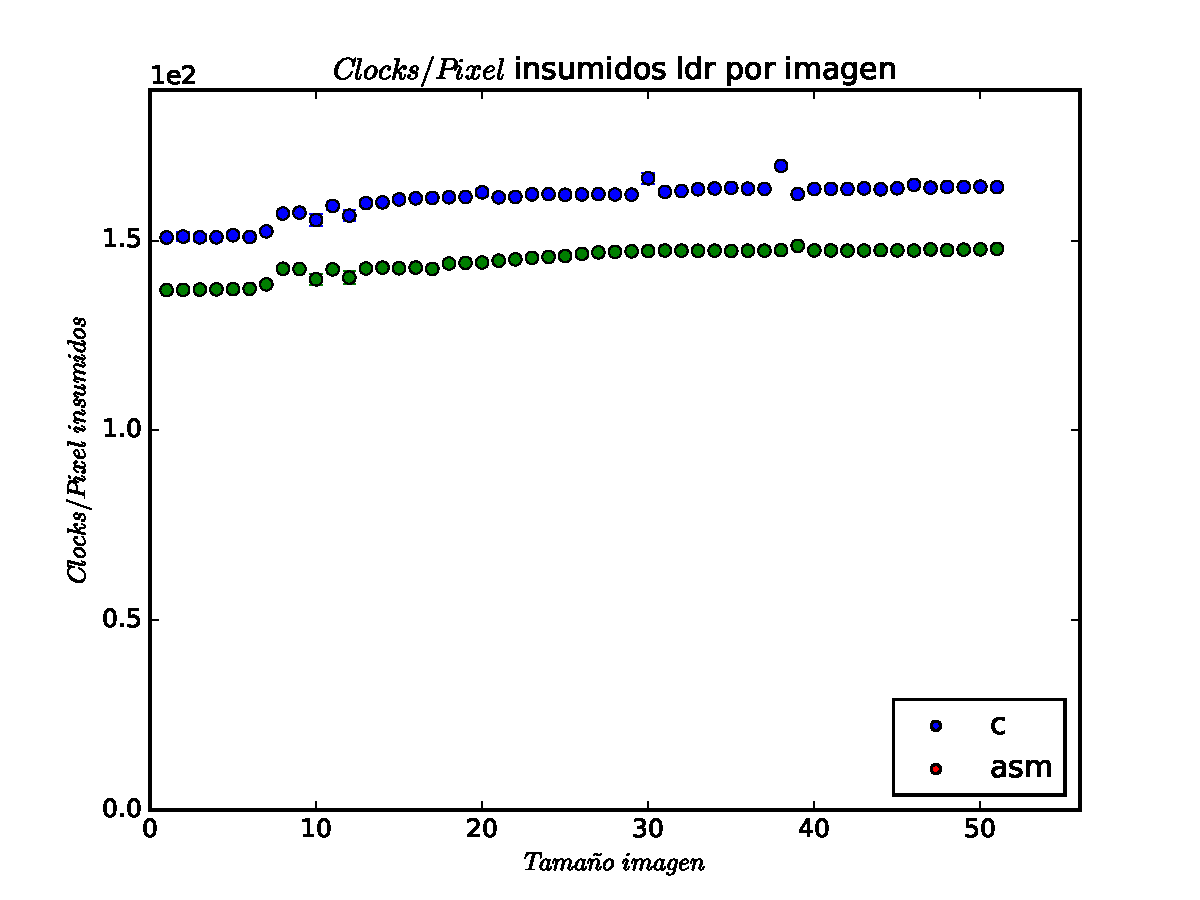
\includegraphics[scale=0.5]{ldrall.pdf}
  \end{center}
\end{figure}

\begin{figure}
  \begin{center}
	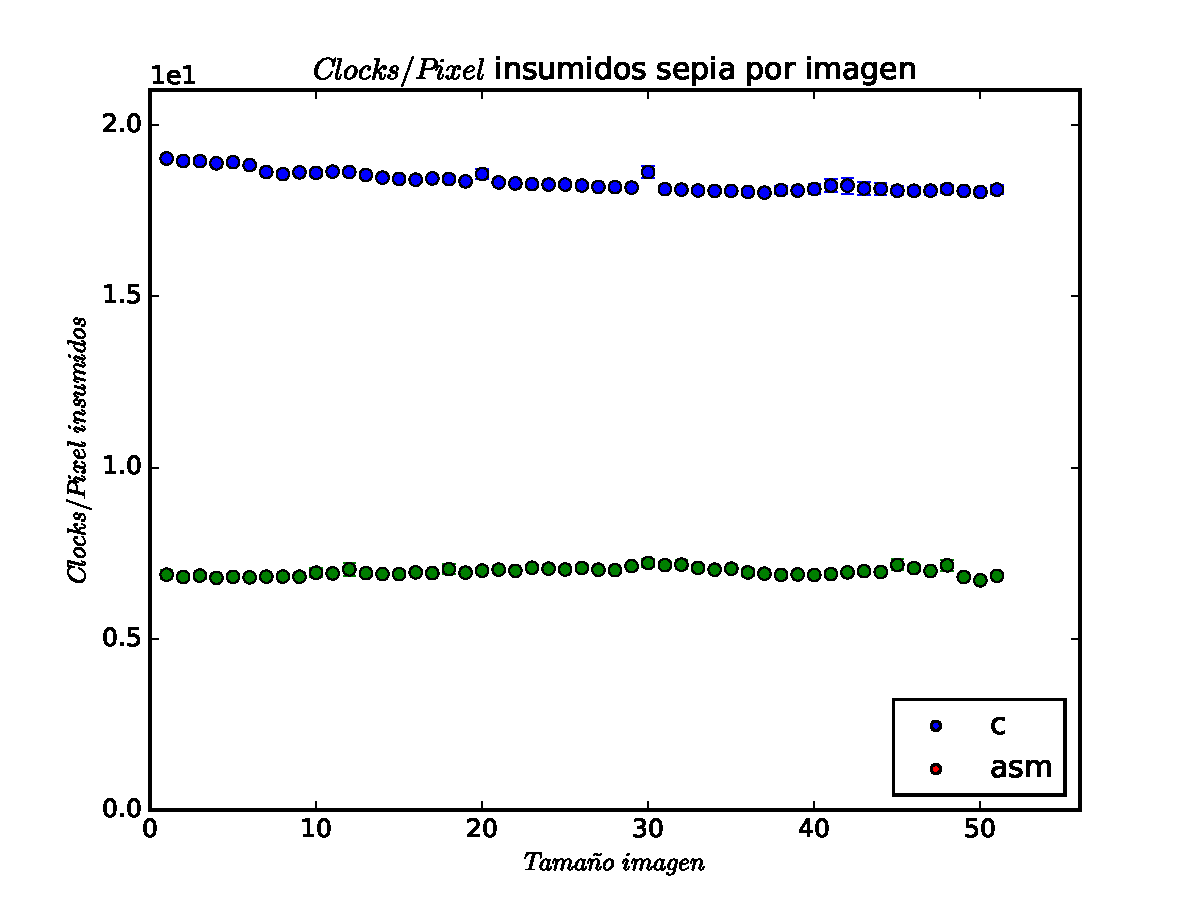
\includegraphics[scale=0.5]{sepiaall.pdf}
  \end{center}
\end{figure}

\begin{figure}
  \begin{center}
	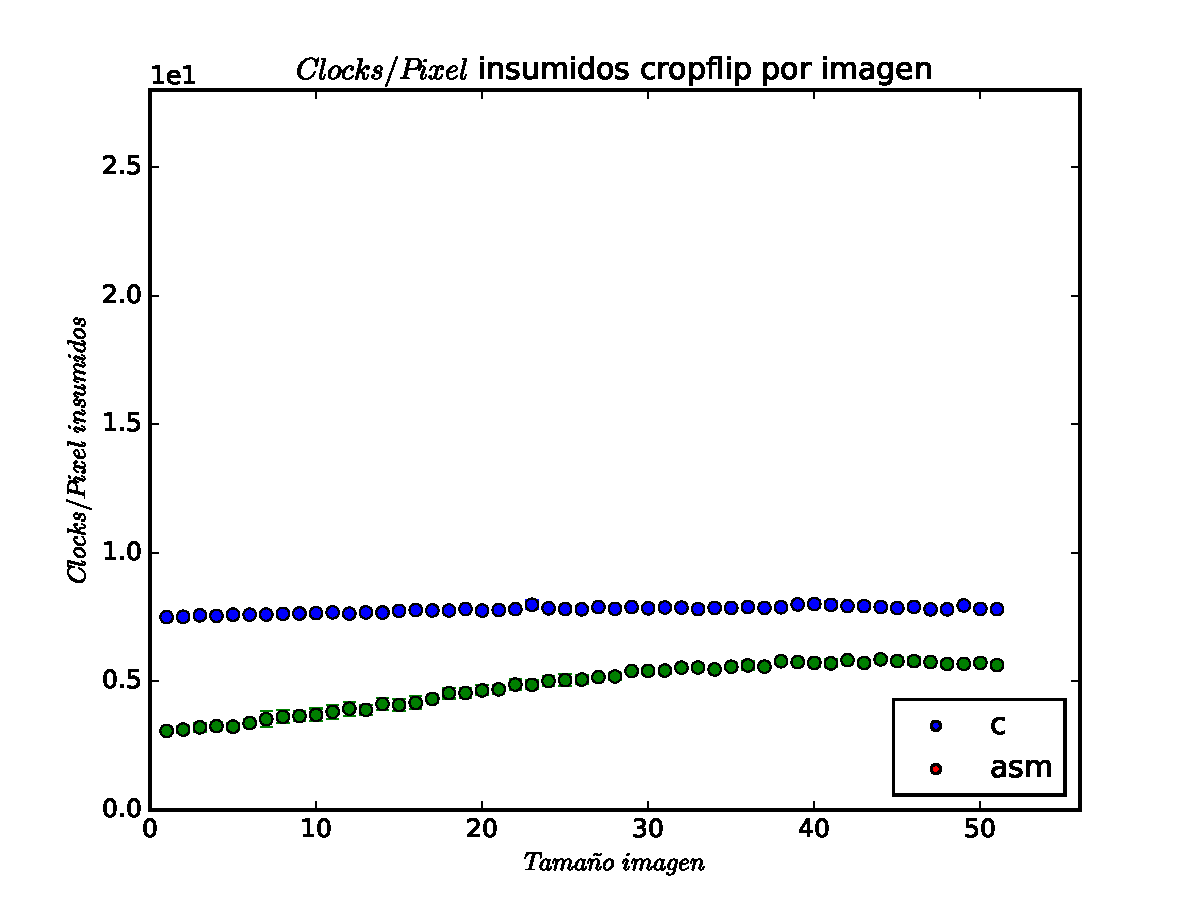
\includegraphics[scale=0.5]{cropflipall.pdf}
  \end{center}
\end{figure}

Puede comprobarse que las mediciones se mantienen comparativamente constantes tanto en la version de $assembler$ $SIMD$ como en $C-O1$
Esto se corresponde con nuestra hipótesis inicial de que aumentos lineales en la cantidad de pixeles se corresponden con aumentos lineales en la cantidad de tiempo total, y que en particular por pixel el tiempo se mantiene aproximadamente constante como muestran los gráficos.



